\documentclass{standalone}

\usepackage{graphicx}
\usepackage{color}
\usepackage{tikz}
\usepackage{psfrag}
\usepackage{subfig}

% Just for this example
\newcommand{\img}{\includegraphics[width=.15\linewidth,height=20pt]{example-image}}

\usepackage{multirow}

\begin{document}



%\begin{tabular}{ *2{c} }
%	\includegraphics[]{A1.pdf} 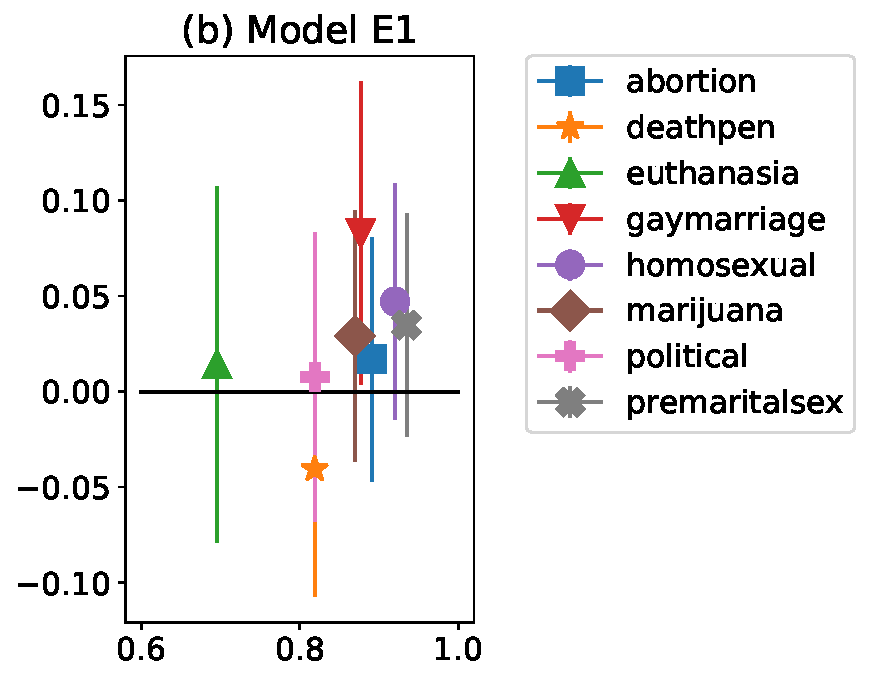
\includegraphics[]{E1.pdf} &
%	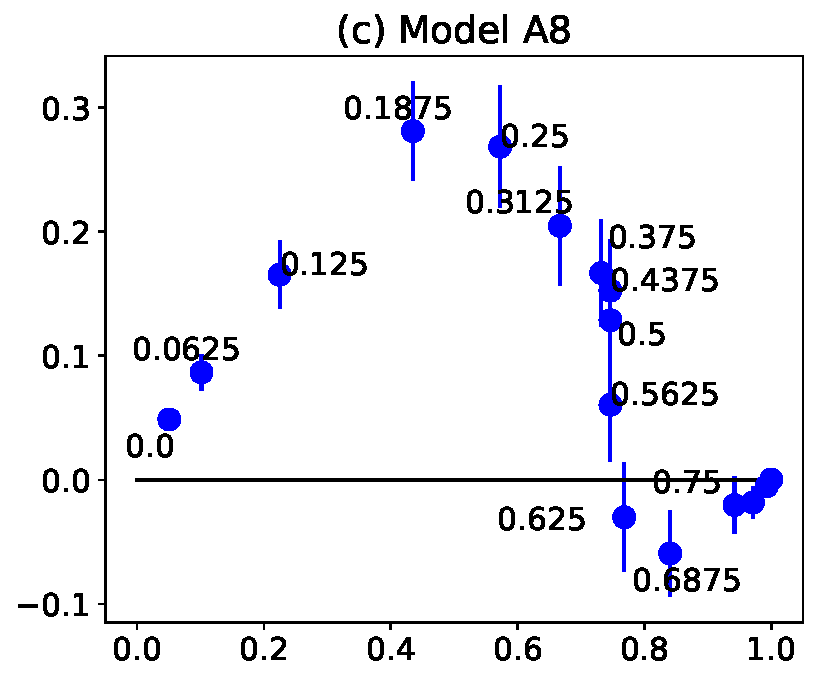
\includegraphics{modelA8v2.pdf} \\
%	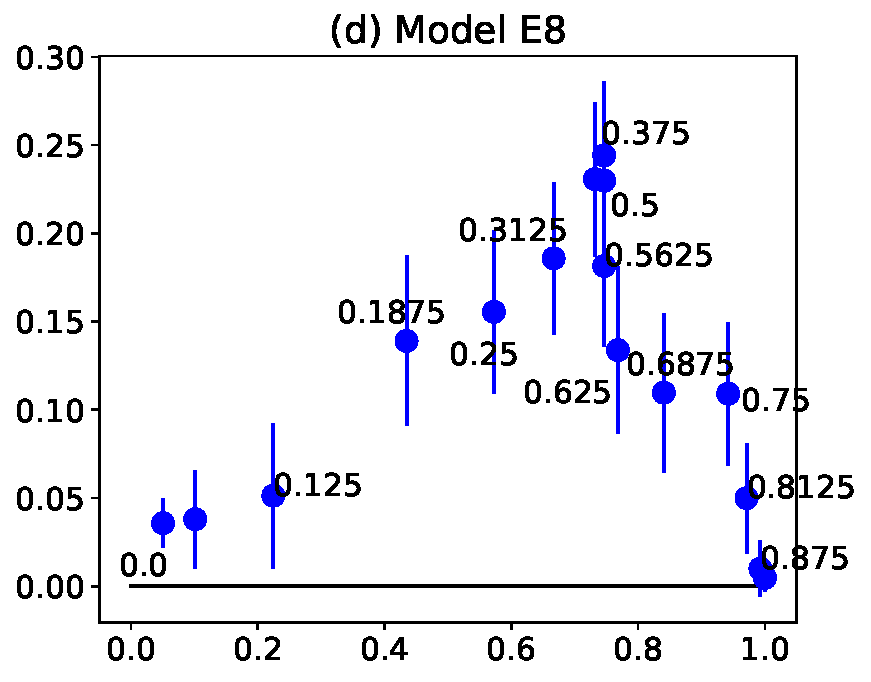
\includegraphics[]{modelE8v2.pdf} &  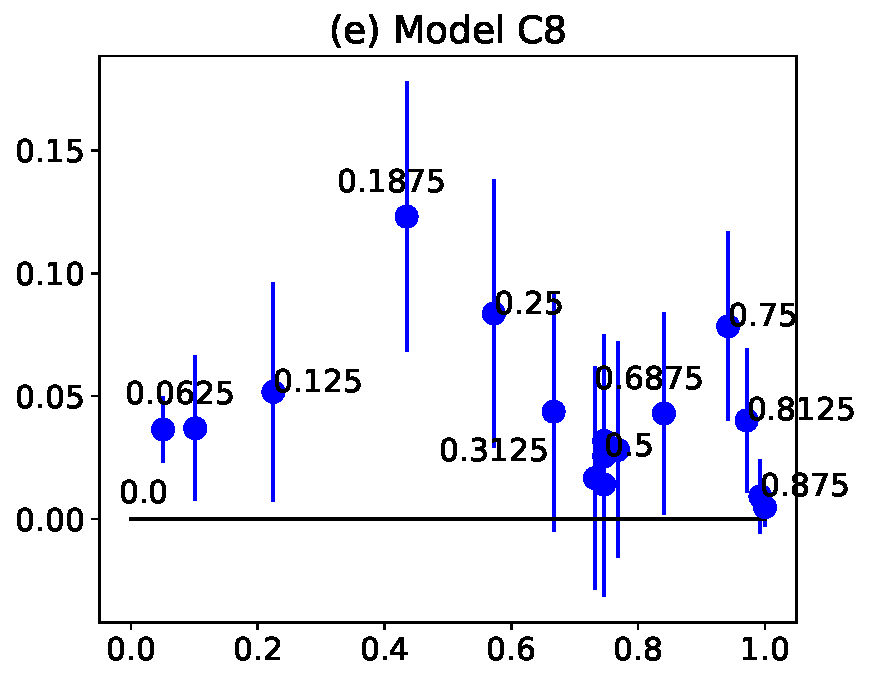
\includegraphics[]{modelC8v2.pdf} 
%\end{tabular}

\begin{tabular} {cc}
	\multirow{2}{*}[10pt]{\rotatebox{90}{$p_D-p_M$}}
		%  \raisebox{.5\normalbaselineskip}[0pt][0pt]{\rotatebox[origin=c]{90}{Scenario A}} 
		&
		\includegraphics[height=5cm]{A1.pdf} 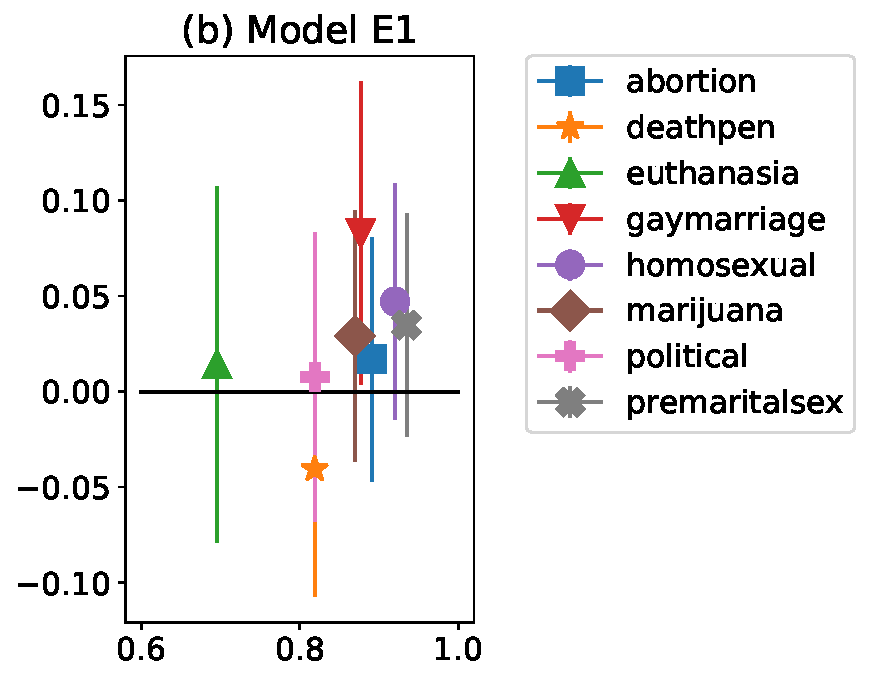
\includegraphics[height=5cm]{E1.pdf}
		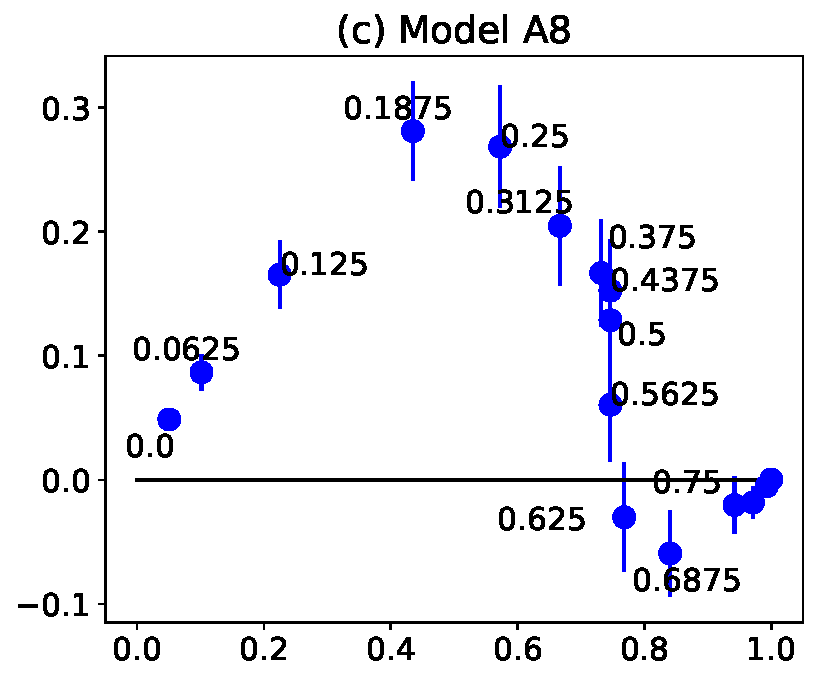
\includegraphics[height=5cm]{modelA8v2.pdf} \\
		 &
		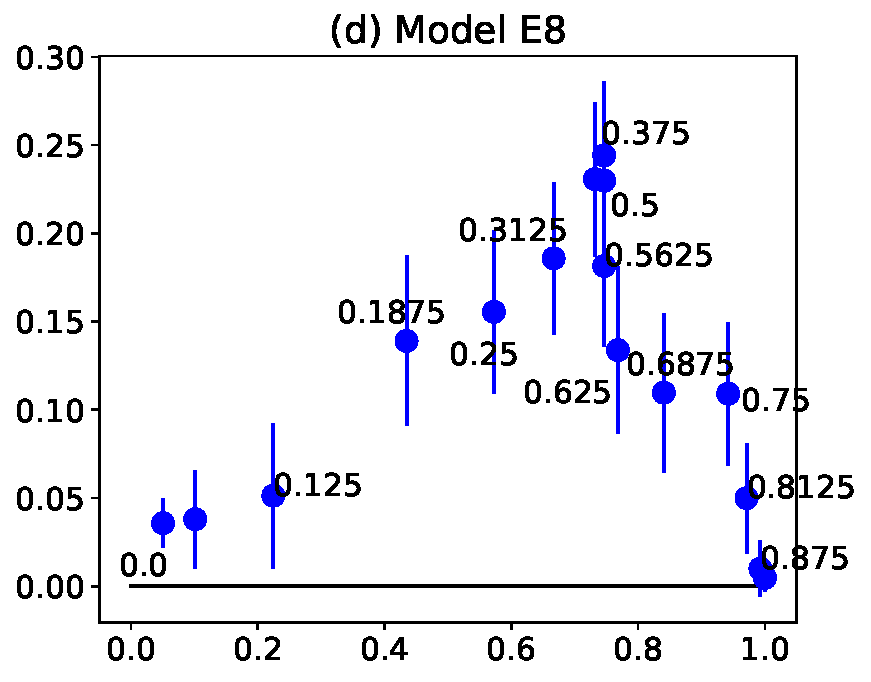
\includegraphics[height=5cm]{modelE8v2.pdf}  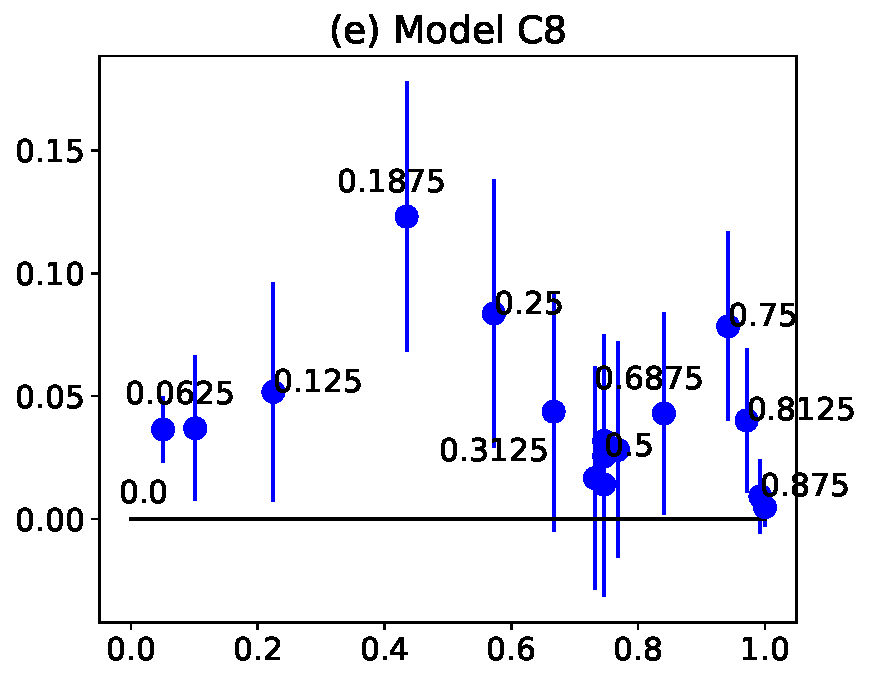
\includegraphics[height=5cm]{modelC8v2.pdf} \\
		& $p_D$
\end{tabular}

\end{document}
